% Solução inicial: todos ligados diretamente à raiz (viável, mas cara)
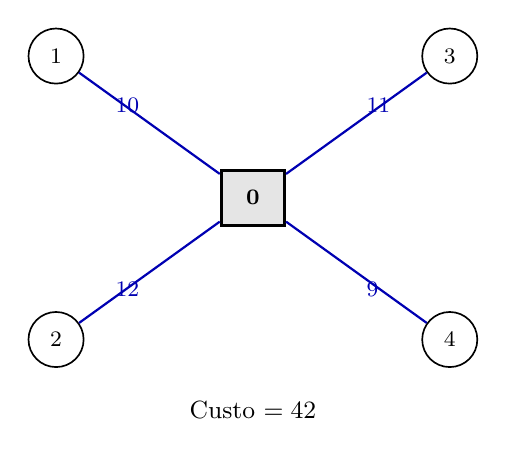
\begin{tikzpicture}
\tikzset{
    >=stealth,
    aresta/.style={-, thick, blue!70!black},
    vertice/.style={circle, semithick, draw=black, inner sep=0pt, minimum size=0.7cm},
    raiz/.style={rectangle, very thick, draw=black, fill=gray!20,
                 minimum width=0.8cm, minimum height=0.7cm}
}
\node[raiz]    (v0) at (2.5, 2)   {\footnotesize \textbf{0}};
\node[vertice] (v1) at (0,   3.8) {\footnotesize 1};
\node[vertice] (v2) at (0,   0.2) {\footnotesize 2};
\node[vertice] (v3) at (5,   3.8) {\footnotesize 3};
\node[vertice] (v4) at (5,   0.2) {\footnotesize 4};
\draw[aresta] (v0) -- node[above left,  font=\footnotesize] {10} (v1);
\draw[aresta] (v0) -- node[below left,  font=\footnotesize] {12} (v2);
\draw[aresta] (v0) -- node[above right, font=\footnotesize] {11} (v3);
\draw[aresta] (v0) -- node[below right, font=\footnotesize] {9}  (v4);
\node[font=\small, align=center] at (2.5,-0.7) {Custo $= 42$};
\end{tikzpicture}
